% Final project report. Compile with pdfLaTeX on Overleaf.
% Upload this file together with the folder figures/ (fig_main_results.pdf, fig_leakage.pdf, fig_missing.pdf).
% If figures show only as framed file names, Overleaf is compiling in draft mode:
% Recompile menu -> Compile mode -> Normal. ([final] below also forces images in draft mode.)
% Every number in this report is copied from the result files written by the code
% (results/summary.md, clip/results/{main,significance,missing}.md, vlm/qwen3vl4b/*).
\documentclass[11pt,a4paper]{article}

\usepackage[margin=2.3cm]{geometry}
\usepackage[T5,T1]{fontenc}   % T5: Vietnamese glyphs for author names (vntex, in Overleaf's TeX Live); T1 stays the main encoding
\usepackage[utf8]{inputenc}
\usepackage{lmodern}
\usepackage{microtype}
\usepackage{amsmath,amssymb}
\usepackage[final]{graphicx}
\usepackage[section]{placeins}  % floats never move past the next section
\usepackage{booktabs}
\usepackage{tabularx}
\usepackage{multirow}
\usepackage{xcolor}
\usepackage{enumitem}
\usepackage{caption}
\usepackage[hidelinks]{hyperref}

\setlist{itemsep=2pt,topsep=4pt}
\captionsetup{font=small,labelfont=bf}
\newcommand{\todo}[1]{\textcolor{red}{[#1]}}   % placeholders to replace before submission
\newcommand{\best}[1]{\textbf{#1}}
\newcommand{\vn}[1]{{\fontencoding{T5}\selectfont #1}}   % Vietnamese names

% ---------------------------------------------------------------------------------
\title{\textbf{Multimodal Food Recognition and\\Information Extraction from Images and Text\\on UPMC Food-101}}
\author{
  Group 12 \quad Topic: \textbf{Multimodal Food Understanding from Images and Text}\\[6pt]
  \vn{Bùi Việt Hoàng} \quad \vn{Vũ Quang Huy} \quad \vn{Nghiêm Trọng Quốc Anh}\\[2pt]
  \vn{Nguyễn Bá Khoa} \quad \vn{Ngô Hải Huyền} \quad \vn{Nguyễn Khắc Hưng}\\[6pt]
  \small Deep Learning, University of Science and Technology of Hanoi (USTH)
}
\date{}

\begin{document}
\maketitle

\begin{abstract}
We study whether combining food photos with their web text improves food recognition and understanding
compared with either modality alone. On UPMC Food-101 (90,678 image--text pairs, 101 dishes) the raw text leaks
the label: a text-only classifier reaches 86\% accuracy by reading dish names. We therefore mask every word of
every class name (\emph{strict} masking) and draw all conclusions in this setting. We compare fine-tuned
baselines (ResNet-50, DistilBERT, TF-IDF, early and late fusion) with light heads on frozen CLIP ViT-B/16
features, including concatenation, gated and cross-attention fusion. With masked text, the best image-only
model reaches 79.06\% and the best text-only model 43.69\%, while cross-attention fusion reaches \best{85.45\%}
(95\% CI 85.01--85.94), $+6.39$ points over the image head (McNemar $p<10^{-160}$). Without text, fusion falls
back to near image-only accuracy; without the image, it drops below the text-only head; stronger modality dropout closes this gap for
cross-attention and narrows it for concatenation. The vision--language model Qwen3-VL-4B extracts dish, cuisine,
ingredients and cooking method as JSON; it needs the image, and the masked text adds no measurable gain. A qualitative error analysis points to label noise,
string-matching evaluation and visually ambiguous plates as the main sources of the remaining errors.
\end{abstract}

% =================================================================================
\section{Introduction and Research Questions}

Food recognition supports dietary logging, recipe search and restaurant applications. Food images on the
web rarely come alone: they are embedded in recipe pages, blog posts or menus that describe the dish, which
suggests a multimodal approach. Our project topic asks us to \emph{recognize food categories and extract useful
information from both food images and related text, and to compare image-only, text-only and multimodal
approaches to determine whether combining both modalities improves food recognition and understanding}.

A naive comparison is misleading on web data, because the text often states the dish name. We therefore first
remove dish names from the text and then ask six research questions:
\begin{description}[leftmargin=1.2cm,style=sameline]
  \item[RQ1] How accurately can 101 dishes be recognized from the image, from the text, and from both?
  \item[RQ2] Is combining both modalities significantly better than either alone once the text no longer
             contains the dish name?
  \item[RQ3] Which fusion strategy works best (late, concatenation, gated, cross-attention), and how do deep
             models compare with TF-IDF and zero-shot CLIP?
  \item[RQ4] How does a fusion model behave when one modality is missing at test time?
  \item[RQ5] Can a vision--language model (VLM) extract dish name, ingredients and cooking method, and which
             input (image, text, both) works best?
  \item[RQ6] How much does label leakage in the text change these conclusions?
\end{description}

\paragraph{Contributions.}
(1) A leakage analysis showing that UPMC Food-101 text contains the label and that results on raw text
overstate the value of text by about 45 points; we use \emph{strict} masking as a fair setting and audit what it
misses. (2) A controlled comparison of four fusion strategies on the same frozen CLIP encoder, plus fine-tuned
baselines, with bootstrap confidence intervals and paired McNemar tests. (3) A missing-modality evaluation.
(4) A structured-extraction pipeline with Qwen3-VL-4B evaluated automatically and by blind manual grading.
(5) An error analysis of classifiers, data and VLM, and an interactive Gradio demo. Code, configuration, result
tables and the scripts that produce every number are in our repository
(\url{https://github.com/viethoang2503/food-recognize-extract}).

% =================================================================================
\section{Related Work}

\paragraph{Food recognition.}
Food-101~\cite{bossard2014food} established a 101-class benchmark of food photos collected from the web.
UPMC Food-101~\cite{wang2015recipe} uses the same 101 classes but pairs each image with the text of the web page
where it was found; it has become a standard benchmark for multimodal classification~\cite{kiela2018efficient}.
To our knowledge, commonly reported results on UPMC Food-101 use the raw text, which contains the dish names
(Section~\ref{sec:res-robust}); such results are not directly comparable with our masked-text results, and the
closer analogue is our \texttt{none} setting.

\paragraph{Multimodal fusion.}
Fusion strategies are commonly grouped into early (feature-level), late (decision-level) and hybrid
fusion~\cite{baltrusaitis2019multimodal}. Late fusion is simple and robust to a missing input but cannot model
interactions between modalities; feature-level fusion can. Gated multimodal units~\cite{arevalo2017gated} learn
per sample how much to trust each modality, and cross-modal attention, popularized by ViLBERT~\cite{lu2019vilbert},
lets the tokens of one modality attend to the other. Randomly dropping a modality during training
(ModDrop~\cite{neverova2016moddrop}) is a standard way to make fusion models usable when an input is missing. We
compare all of these families on one shared encoder, so that differences come from the fusion operator alone.

\paragraph{Pretrained encoders and vision--language models.}
ResNet~\cite{he2016deep} and DistilBERT~\cite{sanh2019distilbert} are standard image and text encoders that are
usually fine-tuned per task. CLIP~\cite{radford2021clip} learns a joint image--text embedding from 400M web pairs
with a contrastive objective and transfers zero-shot to new classification tasks; frozen CLIP features with a small
trained head are a strong and cheap baseline. Instruction-tuned VLMs such as Qwen3-VL~\cite{qwen3vl} accept images
and text and can produce structured answers, which makes them a natural tool for the ``extract useful
information'' part of our topic, where no labeled training data exists.

\paragraph{Evaluation.}
Two classifiers evaluated on the same test images are compared with McNemar's test on the images where exactly one
of them is correct~\cite{mcnemar1947}; we add percentile bootstrap intervals and a Bonferroni correction.

% =================================================================================
\section{Dataset and Data Preparation}
\label{sec:data}

\paragraph{Source, version and split.}
We use UPMC Food-101~\cite{wang2015recipe}. It was released by its authors on the VISIIR project page of
UPMC/LIP6 (\url{http://visiir.lip6.fr/}), which was not reachable when we prepared the data, so we use the public
Kaggle copy \url{https://www.kaggle.com/datasets/gianmarco96/upmcfood101} (\textbf{Version~1}, last updated
2020-10-12, 8.3\,GB, downloaded on 2026-09-30). Each sample is a photo and the text of its source
web page, labeled with one of 101 dishes. The archive ships with a train/test split, which we keep unchanged. We
hold out a stratified 10\% of the official training set as a validation set (seed 42) and drop 26 samples whose
text is empty (Table~\ref{tab:data}). \texttt{DATA.md} in the repository gives the full procedure, and
\texttt{scripts/prepare\_data.py} reproduces the split deterministically.

\begin{table}[!htbp]
\centering
\caption{Dataset after preprocessing.}
\label{tab:data}
\begin{tabular}{lrl}
\toprule
Split & Samples & Origin \\
\midrule
Train & 61,169 & official train folder minus validation \\
Validation & 6,797 & stratified 10\% of the official train folder \\
Test & 22,712 & official test folder (unchanged) \\
\midrule
Total & 90,678 & 90,704 images found, 26 dropped (no text) \\
\bottomrule
\end{tabular}
\end{table}

\paragraph{Preprocessing.}
Images are paired with their texts by file name and split. Texts are cleaned: HTML entities unescaped, HTML tags
and URLs removed, white space collapsed, lower-cased and truncated to 5,000 characters. Images are not modified on
disk; each model applies its own transform (Section~\ref{sec:methods}).

\paragraph{Label leakage and masking.}
The web text frequently names the dish (``\emph{the best chicken wings recipe\ldots}''). A text classifier can
then succeed by string matching rather than by understanding, and any comparison between modalities becomes
unfair. We build three versions of every text:
\begin{itemize}
  \item \texttt{none}: the cleaned text.
  \item \texttt{exact}: every class name of \emph{all} 101 classes (with singular/plural variants) is replaced
        by \texttt{[MASK]}, longest phrase first.
  \item \texttt{strict}: \texttt{exact}, plus every individual word ($\geq$3 letters, excluding stop words) that
        appears in any class name, e.g.\ ``chicken'', ``rice'', ``grilled''.
\end{itemize}
For example, ``grilled chicken with rice'' is unchanged by \texttt{exact} but becomes
``\texttt{[MASK] [MASK]} with \texttt{[MASK]}'' under \texttt{strict}. Masking applies to all classes, not
only the true one, so the mask itself reveals nothing about the label. \textbf{All conclusions in this
report use \texttt{strict}}; \texttt{none} results are shown only to quantify leakage.

\paragraph{What masking removes and what it leaves.}
Because \texttt{strict} masks every word that occurs in any class name, many ingredient and cooking words are
removed too (\emph{chicken, beef, rice, cheese, chocolate, egg, garlic, onion, grilled, fried, French, Greek}), so
text results are a lower bound. Applying our masking function to test phrases shows which cues survive: cuisine
adjectives not used in class names (\emph{Mexican, Italian, Japanese}), ingredients that are not class words
(\emph{avocado, lime, cilantro, basil, mozzarella, tomato, coconut, peanut, soy, noodle, tortilla}) and cooking
words such as \emph{baked, roasted, stir-fry, oven}. For example, ``easy mexican tortilla with avocado lime and
cilantro baked in the oven'' passes unchanged.

\paragraph{Residual leakage.}
Masking matches ASCII class names on word boundaries, so some variants of dish names are \emph{not} masked:
accented spellings (\emph{pho} written with Vietnamese diacritics, \emph{cr\`eme br\^ul\'ee}, \emph{tiramis\`u},
\emph{pa\"ella}), compounds (\emph{cheeseburgers}) and misspellings (\emph{spagetti}). We verified these cases with
the masking code. To estimate how often accented variants occur, we remove diacritics from every masked text and
check whether a class word reappears (\texttt{scripts/report\_stats.py}, section \texttt{leakage\_audit}): although
6.3\% of the test texts contain non-ASCII characters, only 0.07\% (15 of 22,712; 0.12\% of training texts) contain an
accented class name, almost all of them \emph{cr\`eme br\^ul\'ee}. Accent-related leakage is therefore negligible.
Compounds and misspellings are not covered by this audit. The \emph{image} can leak the name too: some photos contain printed text, such as a menu caption
reading ``Chinese Chicken stir-fried rice'' or a restaurant sign ``LOBSTER ME''.

% =================================================================================
\section{Methods}
\label{sec:methods}

\subsection{Baseline methods}

\paragraph{Fine-tuned unimodal models (Milestone 1).}
\textbf{Image}: ResNet-50~\cite{he2016deep} with ImageNet weights, global pooling, dropout 0.2 and a linear
classifier; training augmentation is random resized crop (scale 0.6--1) to 224 px, horizontal flip and color
jitter 0.2, evaluation is resize 256 and center crop 224. \textbf{Text}: DistilBERT-base-uncased~\cite{sanh2019distilbert}
with masked mean pooling, dropout 0.1 and a linear classifier on 256 tokens. \textbf{TF-IDF + logistic
regression}: uni- and bi-grams, 200k features, sublinear term frequency, $C\in\{1,5,20\}$ chosen on validation.

\paragraph{Fusion baselines (Milestone 1).}
\textbf{Late fusion} combines softmax probabilities, $p = w\,p_{\text{img}} + (1-w)\,p_{\text{txt}}$, with
$w\in\{0,0.05,\dots,1\}$ chosen on validation. \textbf{Early fusion} starts from the two unimodal encoders,
projects each to 512 dimensions (LayerNorm, linear, GELU), concatenates them and trains an MLP and both encoders end
to end.

\paragraph{CLIP baselines.}
\textbf{Zero-shot CLIP} needs no training: logits $=100\cos(\mathbf{v},\mathbf{e}_c)$, where $\mathbf{v}$ is the
image embedding and $\mathbf{e}_c$ embeds the prompt ``\emph{a photo of \{class\}, a type of food}''. The
\textbf{CLIP image} and \textbf{CLIP text} heads are MLPs (LayerNorm, dropout, linear to 512, GELU, dropout, linear
to 101) on a single frozen embedding, and \textbf{CLIP late fusion} combines them as above.

\subsection{Main method}

\paragraph{Frozen CLIP features.}
We use CLIP ViT-B/16~\cite{radford2021clip}, frozen and in fp16, and store once for every image and text: a pooled,
L2-normalized embedding $\mathbf{v}\in\mathbb{R}^{512}$ (image) or $\mathbf{t}\in\mathbb{R}^{512}$ (text); 16 image
tokens $\mathbf{V}\in\mathbb{R}^{16\times768}$ (the $14\times14$ patch grid without CLS, average-pooled to
$4\times4$); and 16 text tokens $\mathbf{T}\in\mathbb{R}^{16\times512}$ (the valid tokens, at most 77, split into 16
contiguous chunks and mean-pooled, with a padding mask). All heads are trained on these stored features, so each
run takes minutes.

\paragraph{Feature-level fusion heads.}
Each modality is first projected, $\mathbf{h}_i = \phi_i(\mathbf{v})$, $\mathbf{h}_t=\phi_t(\mathbf{t})$ with
$\phi(\cdot)=\mathrm{GELU}(\mathrm{Linear}(\mathrm{LN}(\cdot)))$ to 512 dimensions.
\textbf{Concat} applies an MLP to $[\mathbf{h}_i;\mathbf{h}_t]$. \textbf{Gated} lets a per-dimension gate decide how
much to trust each modality:
\begin{equation}
  \mathbf{g}=\sigma\!\left(W[\mathbf{h}_i;\mathbf{h}_t]\right),\qquad
  \mathbf{h}=\mathbf{g}\odot\mathbf{h}_i+(1-\mathbf{g})\odot\mathbf{h}_t .
\end{equation}
\textbf{Cross-attention (xattn)}, our main model, lets text tokens attend to image regions. After projecting both
token sets to 256 dimensions and adding learned position embeddings, one pre-norm block computes
\begin{equation}
  \mathbf{Q}' = \mathbf{Q} + \mathrm{MHA}\big(\mathrm{LN}(\mathbf{Q}),\,\mathbf{K},\,\mathbf{K}\big),\qquad
  \mathbf{Q}'' = \mathbf{Q}' + \mathrm{FFN}\big(\mathrm{LN}(\mathbf{Q}')\big),
\end{equation}
with queries $\mathbf{Q}$ from the text tokens, keys/values $\mathbf{K}$ from the image tokens and 4 heads. The
masked mean of $\mathbf{Q}''$ is concatenated with $\mathbf{h}_i$ and $\mathbf{h}_t$ and classified by an MLP.

\paragraph{Modality dropout.}
During training, each sample loses one modality (zeroed features and mask) with probability 0.1, the modality
being chosen uniformly; both are never dropped~\cite{neverova2016moddrop}. The same zeroing simulates a missing
image or text at test time.

\paragraph{Structured extraction with a VLM.}
For the information-extraction part we run Qwen3-VL-4B-Instruct~\cite{qwen3vl} with a system prompt that asks for
exactly one JSON object,
\texttt{\{"dish\_name", "cuisine", "main\_ingredients": [...], "cooking\_method", "confidence"\}}. Three input
modes mirror the classifier comparison: \texttt{image} (photo only), \texttt{text} (strict-masked text only, at most
1,000 characters) and \texttt{image\_text} (both). Outputs are parsed and validated (first JSON object, required
keys, confidence in $[0,1]$); invalid outputs are retried once with the error message. To compute a dish accuracy,
the free-form \texttt{dish\_name} is mapped to a class: if a class name (or a plural variant) appears in it we take
the longest match; otherwise the class with the highest $\max(\text{string ratio},\ \text{word overlap})$, or
\emph{unmapped} if that score is below 0.6.

\paragraph{Demo.}
A Gradio application loads the frozen CLIP encoder and three heads (image, text, \texttt{xattn\_strict}). A user
uploads a photo and optionally types a text, which is cleaned and masked like the training data; the app shows the
top-5 dishes of each branch side by side and can run the VLM to display the extracted JSON.

\subsection{Comparison strategy}
\label{sec:comparison}

\begin{itemize}
  \item \textbf{Same data, same text.} Every model is trained and evaluated on the same split, and all main
        comparisons use \texttt{strict} text.
  \item \textbf{Same encoder for fusion.} The four CLIP fusion strategies share identical frozen features, so their
        differences come from the fusion operator alone; Milestone~1 versus Milestone~2 measures the effect of the
        encoder.
  \item \textbf{Validation-only selection.} Stopping epoch, late-fusion weight $w$ and TF-IDF $C$ are chosen on
        validation; head hyper-parameters (hidden 512, dropout 0.3, attention width 256) were fixed in advance. The
        test split is used once, for reporting.
  \item \textbf{Metrics and uncertainty.} Top-1 accuracy, top-5 accuracy and macro-F1 on 22,712 test images,
        with 95\% percentile bootstrap intervals (1,000 resamples).
  \item \textbf{Paired tests.} Two models are compared on the same images with the paired bootstrap interval of
        the accuracy difference and McNemar's test~\cite{mcnemar1947}; we report Bonferroni-corrected $p$-values
        over all comparisons. A model is called better only if the interval excludes 0 and the corrected $p<0.05$.
  \item \textbf{VLM.} The three VLM modes and the CLIP classifiers are evaluated on the same 200 stratified test
        images. Because ingredients and cooking methods have no ground truth, the authors grade 20 images
        $\times$ 3 modes blind to the mode (rows shuffled, mode in a separate key file), judging from the image:
        dish 0/1, ingredients 0--2, cooking method 0/1. A dish name is correct when it names the dish visible in
        the photo; a more generic but still correct name (``grilled fish'' for grilled salmon) is accepted, a
        different dish is not. Grading was done in a single pass, without inter-rater agreement.
\end{itemize}

% =================================================================================
\section{Experimental Setup}

All experiments run in Google Colab notebooks; features, runs and predictions are resumable and stored on Google
Drive. All neural models use AdamW, a cosine schedule with 5\% warm-up, label smoothing 0.1 and early stopping on
validation accuracy (Table~\ref{tab:hparams}).

\begin{table}[!htbp]
\centering
\caption{Training settings. LR: learning rate (encoder / head). WD: weight decay.}
\label{tab:hparams}
\small
\begin{tabular}{lccccc}
\toprule
Model & Max epochs & Batch & LR & WD & Patience \\
\midrule
ResNet-50 (image) & 10 & 64 & 1e-4 / 1e-3 & 0.05 & 2 \\
DistilBERT (text) & 4 & 32 & 3e-5 / 1e-3 & 0.01 & 2 \\
Early fusion & 4 & 32 & 3e-5 (ResNet), 2e-5 (BERT) / 1e-3 & 0.01 & 2 \\
CLIP heads (all) & 30 & 256 & -- / 1e-3 & 0.01 & 3 \\
\bottomrule
\end{tabular}
\end{table}

\paragraph{Setup 1 --- Baseline vs.\ main model.}
We compare the baselines (fine-tuned ResNet-50, DistilBERT, TF-IDF, Milestone~1 late and early fusion; CLIP
zero-shot; CLIP image, text and late fusion) with the main feature-level CLIP fusion heads (concat, gated,
cross-attention), all with \texttt{strict} text. In early fusion both encoders start from the converged unimodal
runs, so they use lower learning rates (3e-5 for ResNet-50 instead of 1e-4, 2e-5 for DistilBERT instead of 3e-5) to
adapt to fusion without overwriting what they learned. This setup answers RQ3.

\paragraph{Setup 2 --- Main research experiment: image vs.\ text vs.\ both.}
For classification, we compare image-only, text-only and fused models on the 22,712 test images with paired tests
(RQ1, RQ2). For information extraction, Qwen3-VL-4B runs the three modes on the same 200 stratified test images on
one NVIDIA L4 GPU in Colab (bf16 weights, greedy decoding, at most 256 new tokens, images resized to at most 768 px
on the longer side); we report valid-JSON rate, latency, label-based dish accuracy and the manual grades, and score
the CLIP classifiers on the same 200 images (RQ5).

\paragraph{Setup 3 --- Analysis, robustness and ablation.}
(a) \emph{Leakage}: every text and fusion model is also trained and tested with \texttt{none} text (RQ6).
(b) \emph{Missing modality}: each \texttt{strict} fusion model is tested with the text or the image zeroed (RQ4).
(c) \emph{Modality-dropout ablation}: concat and cross-attention are retrained with dropout 0 and 0.3 instead of 0.1.
(d) \emph{Residual-leakage audit} of the masked text (Section~\ref{sec:data}).

% =================================================================================
\section{Results and Discussion}

\subsection{Setup 1: baselines vs.\ main model}

Table~\ref{tab:main} and Figure~\ref{fig:main} give all classifiers with \texttt{strict} text, and
Table~\ref{tab:sig} the paired comparisons.

\begin{table}[!htbp]
\centering
\caption{Test results with \texttt{strict} masking ($n=22{,}712$). CI: 95\% percentile bootstrap interval of
accuracy (1,000 resamples). Best in bold.}
\label{tab:main}
\small
\begin{tabular}{llcccc}
\toprule
Encoder & Model & Accuracy & 95\% CI & Top-5 & Macro-F1 \\
\midrule
\multirow{5}{*}{\shortstack[l]{Milestone 1\\(fine-tuned)}}
 & TF-IDF + LR (text) & 43.69 & 43.07--44.34 & 59.96 & 43.82 \\
 & DistilBERT (text) & 41.42 & 40.78--42.07 & 60.18 & 41.64 \\
 & ResNet-50 (image) & 65.56 & 64.95--66.13 & 84.44 & 65.33 \\
 & Late fusion & 75.63 & 75.08--76.17 & 91.12 & 75.52 \\
 & Early fusion & 77.65 & 77.10--78.19 & 91.35 & 77.58 \\
\midrule
\multirow{7}{*}{\shortstack[l]{Milestone 2\\(frozen CLIP)}}
 & Zero-shot (image) & 71.37 & 70.76--71.97 & 87.33 & 70.66 \\
 & Text head & 38.22 & 37.64--38.83 & 57.13 & 38.28 \\
 & Image head & 79.06 & 78.56--79.57 & 92.51 & 78.95 \\
 & Late fusion & 83.73 & 83.26--84.18 & 95.18 & 83.67 \\
 & Gated fusion & 84.94 & 84.51--85.42 & 95.17 & 84.87 \\
 & Concat fusion & 85.08 & 84.61--85.56 & 95.29 & 85.03 \\
 & Cross-attention fusion & \best{85.45} & 85.01--85.94 & \best{95.49} & \best{85.42} \\
\bottomrule
\end{tabular}
\end{table}

\begin{figure}[!htbp]
\centering
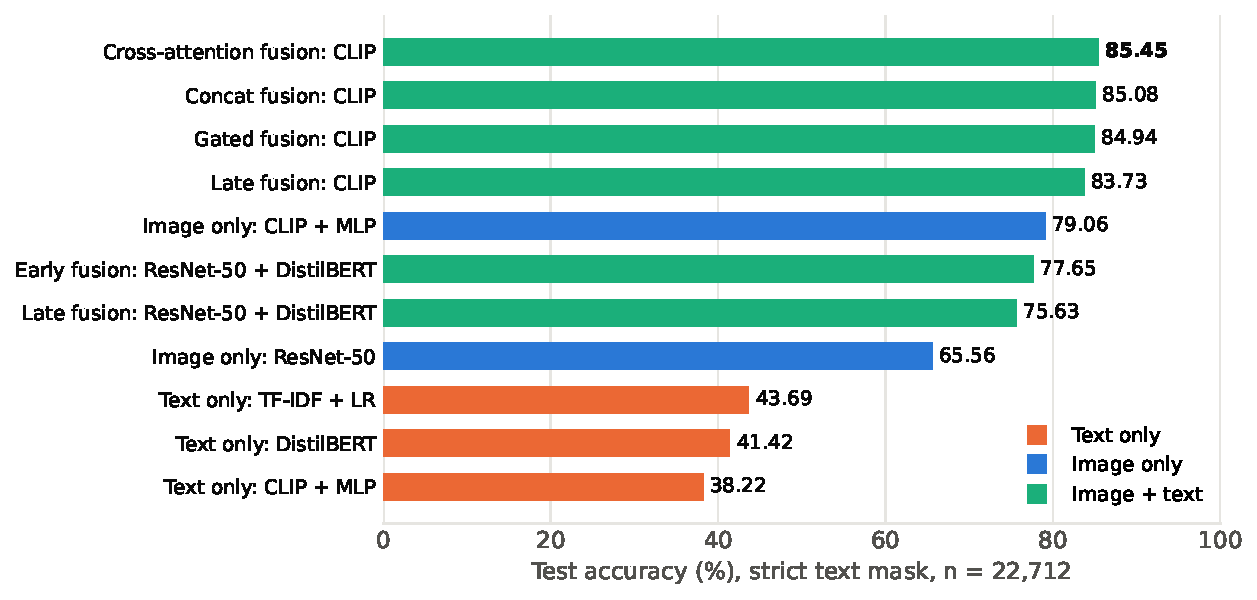
\includegraphics[width=0.92\linewidth]{figures/fig_main_results.pdf}
\caption{Test accuracy of all classifiers with dish names masked in the text (\texttt{strict}).}
\label{fig:main}
\end{figure}

\begin{table}[!htbp]
\centering
\caption{Paired comparisons on the test set. $\Delta = \mathrm{acc}(B)-\mathrm{acc}(A)$ with paired bootstrap
95\% CI; ``A only'' / ``B only'': images correct for one model only; $p$: McNemar; $p_{\text{Bonf}}$: Bonferroni
correction over the 13 comparisons (\texttt{scripts/report\_stats.py}). Values below $10^{-300}$ underflow double
precision and are reported as bounds.}
\label{tab:sig}
\small
\setlength{\tabcolsep}{4pt}
\begin{tabular}{llrcrrll}
\toprule
A & B & $\Delta$ & 95\% CI & A only & B only & $p$ & $p_{\text{Bonf}}$ \\
\midrule
CLIP image & CLIP text & $-40.84$ & $[-41.63, -40.04]$ & 11,025 & 1,750 & $<10^{-300}$ & $<10^{-300}$ \\
CLIP image & xattn & $+6.39$ & $[5.96, 6.84]$ & 664 & 2,115 & $1.5\times10^{-166}$ & $1.9\times10^{-165}$ \\
CLIP text & xattn & $+47.23$ & $[46.50, 47.91]$ & 444 & 11,170 & $<10^{-300}$ & $<10^{-300}$ \\
CLIP late & xattn & $+1.72$ & $[1.34, 2.08]$ & 693 & 1,084 & $2.2\times10^{-20}$ & $2.9\times10^{-19}$ \\
CLIP late & concat & $+1.35$ & $[0.97, 1.71]$ & 717 & 1,024 & $2.2\times10^{-13}$ & $2.9\times10^{-12}$ \\
CLIP late & gated & $+1.21$ & $[0.88, 1.58]$ & 713 & 988 & $3.1\times10^{-11}$ & $4.0\times10^{-10}$ \\
CLIP concat & xattn & $+0.37$ & $[0.07, 0.68]$ & 612 & 696 & $0.022$ & $0.28$ \\
CLIP gated & xattn & $+0.51$ & $[0.17, 0.82]$ & 658 & 774 & $0.0024$ & $0.031$ \\
Zero-shot & CLIP image & $+7.69$ & $[7.22, 8.14]$ & 619 & 2,366 & $4.3\times10^{-224}$ & $5.5\times10^{-223}$ \\
ResNet-50 & Early (M1) & $+12.09$ & $[11.57, 12.72]$ & 1,136 & 3,882 & $<10^{-300}$ & $<10^{-300}$ \\
DistilBERT & Early (M1) & $+36.23$ & $[35.55, 36.89]$ & 422 & 8,651 & $<10^{-300}$ & $<10^{-300}$ \\
Late (M1) & Early (M1) & $+2.02$ & $[1.60, 2.47]$ & 1,043 & 1,502 & $1.1\times10^{-19}$ & $1.4\times10^{-18}$ \\
Early (M1) & xattn & $+7.80$ & $[7.27, 8.26]$ & 827 & 2,598 & $6.2\times10^{-201}$ & $8.1\times10^{-200}$ \\
\bottomrule
\end{tabular}
\end{table}

\paragraph{Which fusion (RQ3)?}
With the encoder fixed, the three feature-level heads are 1.2--1.7 points above late fusion; all three are
significantly better than late fusion (cross-attention $+1.72$, concat $+1.35$, gated $+1.21$ points; Bonferroni
$p\leq4\times10^{-10}$). Late fusion only averages two independent decisions, while the
feature-level heads can learn which text cues matter for which visual pattern. Cross-attention is numerically the
best overall, but its lead over concat ($+0.37$) and gated ($+0.51$) is small: after Bonferroni correction the gain
over gated remains significant while the gain over concat does not. The specific feature-level operator therefore
matters little.

\paragraph{The encoder matters most.}
CLIP cross-attention beats Milestone~1 early fusion by $+7.80$ points, and a small MLP on frozen CLIP image
features beats both CLIP zero-shot ($+7.69$) and a fully fine-tuned ResNet-50 ($+13.5$). CLIP was pretrained on
hundreds of millions of image--text pairs and places both modalities in a shared space, so the expensive part of
the representation is already aligned and the head mostly needs to combine two good summaries. This also explains
why the three feature-level heads land within about 0.5 points of each other. Among text models, the bag-of-words
TF-IDF baseline is best (43.69\%), ahead of DistilBERT (41.42\%) and the CLIP text head (38.22\%), which sees only
77 tokens of a long, noisy page.

\subsection{Setup 2: image vs.\ text vs.\ both}

\paragraph{Classification (RQ1, RQ2).}
With masked text the image is by far the stronger modality (79.06\% with CLIP, 65.56\% with ResNet-50, against
38--44\% for text), yet combining both is significantly better than either: cross-attention fusion beats the image
head by $+6.39$ points (CI 5.96--6.84) and the text head by $+47.23$ points; with fine-tuned encoders, early fusion
beats ResNet-50 by $+12.09$ and DistilBERT by $+36.23$ points (all $p<10^{-160}$). \textbf{Combining image and text
significantly improves recognition, even when the text no longer names the dish.} The two modalities make different
errors: fusion fixes 2,115 of the image head's errors and introduces 664 new ones. What survives masking is mostly
context that is not a class word (cuisine, secondary ingredients, cooking words), which can separate visually
similar dishes; part of the gain may also come from the residual leakage of Section~\ref{sec:data}.

\paragraph{Information extraction (RQ5).}
Tables~\ref{tab:vlm} and~\ref{tab:manual} summarize the VLM. It almost always returns valid JSON (99.5--100\%) in
2.9--3.6\,s per image on the L4 GPU.

\begin{table}[!htbp]
\centering
\caption{Qwen3-VL-4B on 200 stratified test images. Dish accuracy is measured after mapping the free-form dish name
to the 101 classes; invalid and unmapped answers count as wrong. Unmapped: share of \emph{valid} outputs that match
no class (199 valid outputs in text mode, 200 otherwise). Latency per image including retries. For reference, the
CLIP classifiers on the same 200 images reach 76.0\% (image head, CI 70.0--82.0), 38.0\% (text head, 31.5--44.5)
and 80.5\% (cross-attention fusion, 74.5--86.0).}
\label{tab:vlm}
\small
\begin{tabular}{lcccccc}
\toprule
Mode & Valid JSON & Retry & Latency (mean / p90) & Dish acc. & 95\% CI & Unmapped \\
\midrule
Image & 100.0\% & 0.0\% & 3.56 / 4.30 s & 61.0\% & 54.5--67.5 & 24.5\% \\
Text (masked) & 99.5\% & 0.5\% & 2.91 / 3.97 s & 5.5\% & 2.5--9.0 & 79.9\% \\
Image + text & 100.0\% & 0.0\% & 3.57 / 4.26 s & 60.0\% & 53.0--67.0 & 24.5\% \\
\bottomrule
\end{tabular}
\end{table}

\begin{table}[!htbp]
\centering
\caption{Blind manual grading on 20 images (the same images in every mode), judged from the image, next to the
label-based dish accuracy of the same 60 answers. Mean with 95\% percentile bootstrap interval (1,000 resamples,
\texttt{scripts/report\_stats.py}).}
\label{tab:manual}
\small
\setlength{\tabcolsep}{4pt}
\begin{tabular}{lcccc}
\toprule
Mode & Dish, manual (0/1) & Dish, by label & Ingredients (0--2) & Cooking method (0/1) \\
\midrule
Image & 0.80 [0.60, 0.95] & 0.50 [0.30, 0.70] & 1.65 [1.40, 1.90] & 0.90 [0.75, 1.00] \\
Text (masked) & 0.05 [0.00, 0.15] & 0.00 [0.00, 0.00] & 0.10 [0.00, 0.25] & 0.15 [0.00, 0.35] \\
Image + text & 0.85 [0.70, 1.00] & 0.55 [0.35, 0.75] & 1.65 [1.40, 1.90] & 0.90 [0.75, 1.00] \\
\bottomrule
\end{tabular}
\end{table}

\emph{The VLM needs the image.} With masked text only, it identifies 5.5\% of dishes and 79.9\% of its answers match
no class; manual grades are near zero for all fields. With the image, manual grades are high (dish 0.80--0.85,
ingredients 1.65/2, cooking method 0.90). \emph{The masked text does not help it.} Adding the text to the image
changes dish accuracy from 61.0\% to 60.0\% on the same 200 images: 8 images are correct only with the image and 6
only with image and text (paired difference $-1.0$ points, CI $-4.5$ to $+2.5$; McNemar $p=0.79$). In the manual grades they disagree on
the dish for one image out of 20 ($p=1.0$), a borderline name discussed in Section~\ref{sec:errors}. The VLM
already recognizes most dishes from the photo, and the masked text adds little it does not see.
\emph{Classifier versus VLM.} On the same 200 images, the CLIP classifiers score higher on the label-based dish
accuracy (76.0\% image head, 80.5\% fusion, against 61.0\% and 60.0\% for the VLM) \todo{paired test from
report\_stats.py, section vlm\_vs\_classifier: VLM image vs image head, $\Delta$ = ..., McNemar $p$ = ...; VLM
image+text vs xattn, $\Delta$ = ..., $p$ = ...}. Part of this gap comes from the evaluation rather than the model:
the classifiers choose among the 101 known classes, whereas the VLM answers in an open vocabulary that must then be
mapped, and on the graded images its manual dish score (0.80--0.85) is close to the classifiers. The VLM, however,
produces what the classifiers cannot: plausible ingredient lists and cooking methods. For a \emph{guacamole} image
it returns:
\begin{center}
\small
\begin{tabular}{@{}l@{}}
\texttt{\{"dish\_name": "guacamole", "cuisine": "Mexican",} \\
\texttt{\ \ "main\_ingredients": ["avocado", "tomato", "onion", "lime", "cilantro",} \\
\texttt{\ \ \ \ "jalape\~no"], "cooking\_method": "mashed", "confidence": 0.95\}}
\end{tabular}
\end{center}

\subsection{Setup 3: analysis, robustness and ablation}
\label{sec:res-robust}

\paragraph{Label leakage (RQ6).}
Figure~\ref{fig:leak} compares the same models with raw (\texttt{none}) and masked (\texttt{strict}) text. With raw
text, every text model scores about 86\%, \emph{higher than the image}, and fusion reaches 95\%. Masking costs text
models 43--48 points, CLIP fusion heads 9.6--11.1 points and the Milestone~1 fusion models 15.0--17.7 points. On raw
text one would wrongly conclude that text is the more informative modality; this conclusion is an artifact of dish
names in the text. Leakage also inflates the apparent benefit of fusion ($+16$ points over the image instead of
$+6.4$).

\begin{figure}[!htbp]
\centering
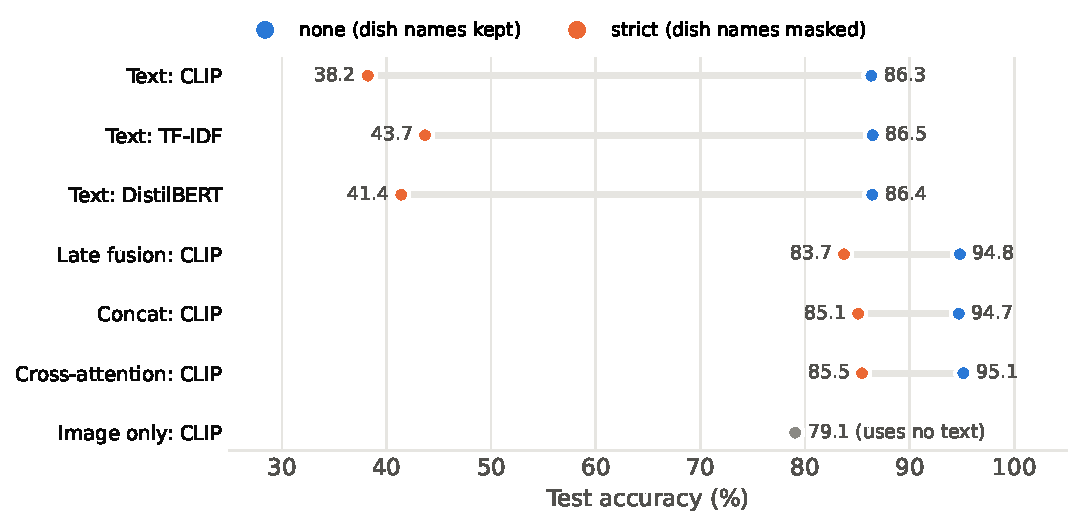
\includegraphics[width=0.9\linewidth]{figures/fig_leakage.pdf}
\caption{Test accuracy with raw text (\texttt{none}) and with dish names masked (\texttt{strict}). DistilBERT is
the Milestone~1 model; the others use frozen CLIP features.}
\label{fig:leak}
\end{figure}

\paragraph{Missing modality (RQ4).}
Without text, the learned fusion heads lose 6.8--7.8 points but stay within 0.9--1.4 points of the dedicated image
head (Table~\ref{tab:missing}, Figure~\ref{fig:missing}). Without the image they fall to 33.8--35.0\%,
\emph{below} the dedicated text head (38.22\%). The heads thus rely mainly on the image: with 10\% modality dropout
the text pathway is rarely trained alone (see the ablation below). Late fusion degrades gracefully by construction (it falls back to the
unimodal heads) but is the weakest when both inputs are present.

\begin{table}[!htbp]
\centering
\caption{Accuracy (\%) with a missing modality at test time (\texttt{strict}). References: image head 79.06,
text head 38.22.}
\label{tab:missing}
\small
\begin{tabular}{lccc}
\toprule
Fusion head & Both & Text removed & Image removed \\
\midrule
Late & 83.73 & 79.06 & 38.22 \\
Concat & 85.08 & 77.78 & 33.82 \\
Gated & 84.94 & 78.17 & 33.76 \\
Cross-attention & 85.45 & 77.70 & 34.96 \\
\bottomrule
\end{tabular}
\end{table}

\begin{figure}[!htbp]
\centering
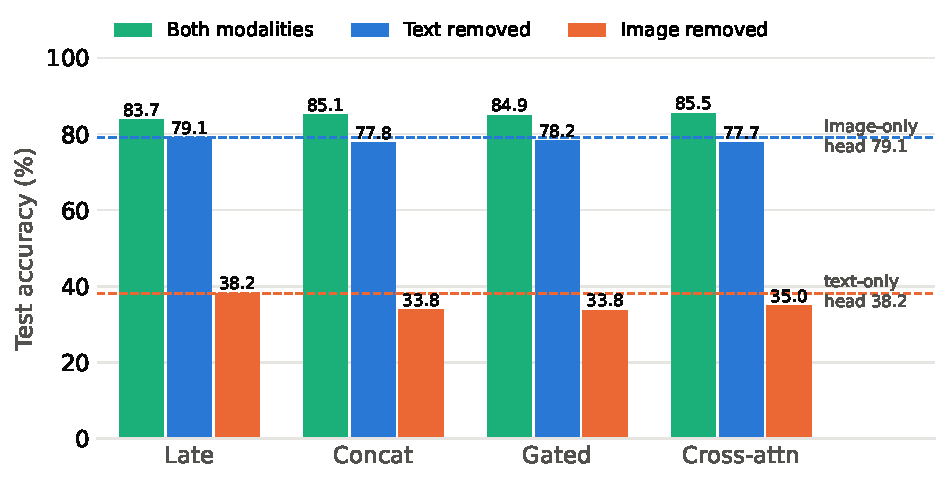
\includegraphics[width=0.85\linewidth]{figures/fig_missing.pdf}
\caption{Fusion heads with both modalities, without text, and without image. Dashed lines: dedicated unimodal heads.}
\label{fig:missing}
\end{figure}

\paragraph{Modality-dropout ablation.}
Table~\ref{tab:md} retrains concat and cross-attention with modality dropout 0 and 0.3. Without dropout, the heads
collapse when an input is missing (cross-attention: 23.95\% without the image, 72.87\% without text). Raising the
rate steadily improves both missing-modality conditions: at 0.3, cross-attention reaches 38.58\% without the image,
on par with the dedicated text head (38.22\%), and 78.34\% without text, close to the image head (79.06\%). For concat, 0.3 narrows the image-removed gap
(36.86\%) but does not close it. With both inputs, each head's accuracy changes by at most 0.21 points across the
three rates, well inside the confidence intervals (we did not run paired tests for these runs). Modality dropout
thus buys robustness with no measurable cost, and 0.3 looks like a better default than our 0.1; since this rate
was chosen after seeing test results, a validation-based choice would be needed to confirm it.

\begin{table}[!htbp]
\centering
\caption{Modality-dropout ablation (\texttt{strict}, accuracy in \%). References: image head 79.06, text head 38.22.}
\label{tab:md}
\small
\begin{tabular}{lcccc}
\toprule
Head & Dropout & Both & Text removed & Image removed \\
\midrule
\multirow{3}{*}{Concat} & 0 & 84.87 & 75.36 & 24.78 \\
 & 0.1 & 85.08 & 77.78 & 33.82 \\
 & 0.3 & 85.08 & 78.45 & 36.86 \\
\midrule
\multirow{3}{*}{Cross-attention} & 0 & 85.35 & 72.87 & 23.95 \\
 & 0.1 & 85.45 & 77.70 & 34.96 \\
 & 0.3 & 85.44 & 78.34 & 38.58 \\
\bottomrule
\end{tabular}
\end{table}

\paragraph{Practical implication.}
For a deployed system the image should be treated as the primary input. Fusion is worth adding when text is
available, but it should be trained with enough modality dropout (0.3 here) so that it degrades gracefully, and it
can still over-trust unusual text (Section~\ref{sec:errors}).

% =================================================================================
\section{Error and Qualitative Analysis}
\label{sec:errors}

Table~\ref{tab:errors} lists representative error cases found in the graded VLM sample, the demo and the masking
audit; the paragraphs below explain their causes.

\begin{table}[!htbp]
\centering
\caption{Representative error cases and their causes.}
\label{tab:errors}
\small
\begin{tabularx}{\linewidth}{l>{\raggedright\arraybackslash}X>{\raggedright\arraybackslash}X}
\toprule
Source & Case & Cause \\
\midrule
Dataset & Image labeled \emph{poutine} shows glazed doughnuts; \emph{ramen} shows roast beef & Wrong web label; the
VLM is right (``Caramelized Doughnut Sticks'', ``Roast Beef'') but scored wrong by label \\
Dataset & Images with no food (a T-shirt, a restaurant interior) & Web noise; the VLM answers ``unknown'' or a word
printed in the image, with confidence 0.1 \\
VLM, image & \emph{beef\_tartare} described as ``Crispy Fish with Herb Pur\'ee'' (confidence 0.85) & Breaded croquettes and
quinoa crumbs on the plate look like fried fish; the raw tartare, the largest item, is missed \\
VLM, image & \emph{beet\_salad} described as ``Roasted Butternut Squash'' & Yellow beet cubes look like squash;
visually ambiguous ingredient \\
VLM, mapping & ``Fish Cakes'' (crab cakes) mapped to \emph{cup\_cakes} & String similarity on the generic word
``cakes'' \\
VLM, grading & Same fried-rice photo: ``Asian-style rice salad'' (0) vs ``Ginger Beef Rice'' (1) & Borderline name;
the only image vs image+text disagreement \\
VLM, text & 79.9\% unmapped answers; ``sushi'' for a ramen label & Masked text alone does not identify the dish \\
VLM, language & ``honey'' written in Chinese characters & Drift from the English-only instruction \\
Demo & Vietnamese caption pushes fusion to \emph{pho} (33\%) though the image head says \emph{pizza} (80\%) &
Out-of-domain text; possibly an accented dish name that escapes the mask \\
\bottomrule
\end{tabularx}
\end{table}

\paragraph{Errors that come from the data.}
Part of what is counted as error is not a model failure. UPMC labels come from web search, and some test images are
mislabeled or contain no food; on these, a correct prediction is scored wrong. Printed text inside images (a menu
caption, a ``LOBSTER ME'' sign) can also give the dish away to image models, which inflates rather than lowers
accuracy. Both effects mean that the reported accuracies are approximate, and that small differences between
models should not be over-interpreted.

\paragraph{Errors that come from the evaluation.}
The VLM's label-based dish accuracy is much lower than its manual grade: on the same 20 images and answers, 80--85\%
of the dish names are correct judged from the image but only 50--55\% after mapping to the label
(Table~\ref{tab:manual}); over all 60 graded answers, 56.7\% versus 35.0\%. Two causes explain the gap: the mapping
fails on 24.5\% of answers or picks a wrong class from a generic word, and some labels are wrong. Manual grading
has its own limits: names such as ``Asian-style rice salad'' for fried rice are judgment calls, and the single
image where the image and image+text modes disagree is exactly such a case.

\paragraph{Classifier errors.}
\todo{Table: top-5 confused pairs of xattn\_strict (report\_stats.py, classifier\_confused\_xattn) and the five
classes most helped / hurt by adding text (classifier\_text\_gain), with two sentences on why: visually similar
dishes, and which classes the masked text helps.}

\paragraph{Errors that come from the models.}
The VLM's real errors are confident misidentifications of visually ambiguous plates (breaded croquettes read as fried
fish next to a raw tartare, squash versus yellow beet) and occasional language drift. For the classifiers, fusion fixes 2,115 of
the image head's errors but introduces 664 new ones: when the masked text points to the wrong dish, the fusion head
can follow it. The demo shows an extreme case. A Vietnamese caption pushed the fusion head toward \emph{pho} while
the image head correctly predicted \emph{pizza}. A possible cause is the masking gap of Section~\ref{sec:data}:
Vietnamese writes the dish name with diacritics, which \texttt{strict} does not mask, so the head may have received
an almost explicit dish name. Such text is essentially absent from the corpus (the audit finds no accented
\emph{pho} at all), so the head never learned how much to trust it. We did not record the masked caption, so this
remains a hypothesis.

% =================================================================================
\section{Conclusion and Limitations}

On UPMC Food-101, the web text leaks the label, and evaluating on raw text would wrongly suggest that text is the
stronger modality. With dish names masked, the image is the primary signal (79.06\%) and text alone is weak
(43.69\% at best), yet combining them is significantly better than either: cross-attention fusion on frozen CLIP
features reaches 85.45\% accuracy and 95.49\% top-5, $+6.39$ points over the image head. Feature-level fusion is
1.2--1.7 points above late fusion, the specific operator matters little, and the pretrained encoder matters most.
Fusion models lean on the image; with 10\% modality dropout they fall below the text-only head when the image is
missing, and raising the rate to 0.3 closes this gap for cross-attention and narrows it for concatenation, with no
measurable cost when both inputs are present. Beyond the class label, a 4B-parameter VLM extracts
usable ingredients and cooking methods from the photo, but it needs the image, and the masked text adds nothing
measurable.

\paragraph{Limitations.}
All runs use one training seed, so intervals reflect only test-set sampling. \texttt{strict} masking over-masks
some descriptive words, while compound and misspelled dish names and text printed in images can still leak (accented
names affect only 0.07\% of test texts).
Text budgets differ (CLIP 77 tokens, DistilBERT 256, TF-IDF up to 5,000 characters, the VLM 1,000 characters).
Labels are noisy, we did not check for duplicate images across splits, and UPMC images may be part of CLIP's or
Qwen3-VL's pretraining data. The VLM evaluation is small (200 images, 20 graded per mode, one grading pass) and its
label-based accuracy depends on string matching. Future work: more seeds, accent-folding and fuzzy matching in the mask,
partial fine-tuning of CLIP, letting the VLM choose among the classifier's top-5 candidates, and larger VLMs.

% =================================================================================
\begin{thebibliography}{99}\small

\bibitem{arevalo2017gated}
J.~Arevalo, T.~Solorio, M.~Montes-y-G\'omez, and F.~A. Gonz\'alez.
\newblock Gated multimodal units for information fusion.
\newblock In \emph{ICLR Workshop}, 2017.

\bibitem{baltrusaitis2019multimodal}
T.~Baltru\v{s}aitis, C.~Ahuja, and L.-P. Morency.
\newblock Multimodal machine learning: A survey and taxonomy.
\newblock \emph{IEEE TPAMI}, 41(2):423--443, 2019.

\bibitem{bossard2014food}
L.~Bossard, M.~Guillaumin, and L.~Van~Gool.
\newblock Food-101 -- Mining discriminative components with random forests.
\newblock In \emph{ECCV}, 2014.

\bibitem{he2016deep}
K.~He, X.~Zhang, S.~Ren, and J.~Sun.
\newblock Deep residual learning for image recognition.
\newblock In \emph{CVPR}, 2016.

\bibitem{kiela2018efficient}
D.~Kiela, E.~Grave, A.~Joulin, and T.~Mikolov.
\newblock Efficient large-scale multi-modal classification.
\newblock In \emph{AAAI}, 2018.

\bibitem{lu2019vilbert}
J.~Lu, D.~Batra, D.~Parikh, and S.~Lee.
\newblock {ViLBERT}: Pretraining task-agnostic visiolinguistic representations for vision-and-language tasks.
\newblock In \emph{NeurIPS}, 2019.

\bibitem{mcnemar1947}
Q.~McNemar.
\newblock Note on the sampling error of the difference between correlated proportions or percentages.
\newblock \emph{Psychometrika}, 12(2):153--157, 1947.

\bibitem{neverova2016moddrop}
N.~Neverova, C.~Wolf, G.~Taylor, and F.~Nebout.
\newblock {ModDrop}: Adaptive multi-modal gesture recognition.
\newblock \emph{IEEE TPAMI}, 38(8):1692--1706, 2016.

\bibitem{qwen3vl}
Qwen Team.
\newblock Qwen3-VL-4B-Instruct.
\newblock Model card, \url{https://huggingface.co/Qwen/Qwen3-VL-4B-Instruct}, 2025.

\bibitem{radford2021clip}
A.~Radford, J.~W. Kim, C.~Hallacy, A.~Ramesh, G.~Goh, S.~Agarwal, G.~Sastry, A.~Askell, P.~Mishkin, J.~Clark,
G.~Krueger, and I.~Sutskever.
\newblock Learning transferable visual models from natural language supervision.
\newblock In \emph{ICML}, 2021.

\bibitem{sanh2019distilbert}
V.~Sanh, L.~Debut, J.~Chaumond, and T.~Wolf.
\newblock {DistilBERT}, a distilled version of {BERT}: smaller, faster, cheaper and lighter.
\newblock \emph{arXiv:1910.01108}, 2019.

\bibitem{wang2015recipe}
X.~Wang, D.~Kumar, N.~Thome, M.~Cord, and F.~Precioso.
\newblock Recipe recognition with large multimodal food dataset.
\newblock In \emph{IEEE ICME Workshops}, 2015.

\end{thebibliography}

% =================================================================================
\clearpage
\appendix
\section{Member Contributions}

\begin{table}[!htbp]
\centering
\caption{Contribution of each member.}
\label{tab:contrib}
\small
\begin{tabularx}{\linewidth}{lX}
\toprule
Member & Contribution \\
\midrule
\vn{Bùi Việt Hoàng} & \todo{tasks} \\
\vn{Vũ Quang Huy} & \todo{tasks} \\
\vn{Nghiêm Trọng Quốc Anh} & \todo{tasks} \\
\vn{Nguyễn Bá Khoa} & \todo{tasks} \\
\vn{Ngô Hải Huyền} & \todo{tasks} \\
\vn{Nguyễn Khắc Hưng} & \todo{tasks} \\
\bottomrule
\end{tabularx}
\end{table}

\section{Reproducibility}

Code, configuration (\texttt{configs/default.yaml}) and notebooks:
\url{https://github.com/viethoang2503/food-recognize-extract}. Data source, version, split and preprocessing:
\texttt{DATA.md}. The scripts write all run outputs to Google Drive; copies of the result tables quoted here are in
\texttt{docs/results/}, and the additional statistics (Bonferroni correction, Milestone~1 intervals, leakage audit,
paired VLM tests, manual-grade intervals) are computed by \texttt{scripts/report\_stats.py}. Demo: \todo{Demo link}.
Each script skips finished runs and resumes interrupted ones.

\begin{center}
\small
\begin{tabularx}{\linewidth}{lX}
\toprule
Step & Command (notebook) \\
\midrule
Data & \texttt{prepare\_data.py} --- manifest, splits, masked texts (01) \\
Milestone 1 & \texttt{train\_tfidf.py}, \texttt{train.py -{}-modality image|text|multimodal}, \texttt{late\_fusion.py}, \texttt{summarize.py} (01) \\
Milestone 2 & \texttt{extract\_clip.py}, \texttt{run\_clip\_suite.py}, \texttt{summarize\_clip.py} (02) \\
Ablation & \texttt{train\_head.py -{}-head concat|xattn} with \texttt{head.modality\_dropout=0} or \texttt{0.3} (02) \\
VLM & \texttt{vlm\_extract.py -{}-mode image|text|image\_text}, \texttt{vlm\_evaluate.py} (03) \\
Report statistics & \texttt{report\_stats.py} (after the steps above) \\
Demo & \texttt{build\_demo\_examples.py}, \texttt{demo.py -{}-share} (04) \\
\bottomrule
\end{tabularx}
\end{center}

\end{document}
